\chapter{Phân tích và đặc tả yêu cầu}

\section{Đặc tả yêu cầu hệ thống}
\subsection{Phạm vi}
\subsubsection{Tổng quát}
Khách hàng của ứng dụng này là Trung tâm quản lý và điều hành vận tải hành khách công cộng. Nhóm chúng tôi thực hiện một trang web như là cổng thông tin về tình hình giao thông tại thành phố Hồ Chí Minh kết hợp chức năng giám sát để hỗ trợ quản lí tình hình giao thông trong thành phố trên nền tảng ứng dụng bản đồ.

Thông tin về tình hình giao thông được cung cấp bởi camera lưu động gắn trên các phương tiện vận tải hành khách nên phạm vi được giám sát là những tuyến đường nội thành có xe buýt đi ngang.

SBT sẽ bao gồm 2 chức năng tương ứng với 2 đối tượng sử dụng: xem tình hình giao thông (đối với khách) và giám sát, xác nhận tình hình giao thông (đối với admin).

Trong tài tài liệu này nói chung và trong chương này nói riêng, chúng tôi chủ yếu giới hạn phạm vi nội dung là các chức năng giám sát của admin và các vấn đề liên quan tới những chức năng này.

\subsubsection{Mục tiêu của hệ thống}
Mục tiêu của dự án này là:

\begin{itemize}
	\item Hiện thực chức năng admin của hệ thống giám sát giao thông nền web.
	\item Thu thập và biểu diễn thông tin từ hàng ngàn camera được gắn trên hệ thống phương tiện giao thông công cộng trong nội thành thành phố HCM dưới dạng live-stream video.
	\item Tính toán vận tốc lưu thông tại mọi vị trí từ nguồn thu thập được và thể hiện trên bản đồ, đồng thời phân tích và dự báo khả năng xảy ra kẹt xe trên phạm vi toàn thành phố.
	\item Thông báo cho người quản trị hệ thống về khả năng xảy ra kẹt xe và yêu cầu họ xác thực thông tin bằng cách xem video. Thông tin đã được xác thực sau đó sẽ được lưu lại và công bố đến mọi người truy cập vào website sau đó.
	\item Vì thông tin được công bố trên website là thông tin mang tính tức thời và được xác minh bởi người quản trị nên rất đáng tin cậy. Nó sẽ giúp mọi người tham gia giao thông chọn được cho mình lộ trình an toàn, thông thoáng để lưu thông nhanh chóng một cách tiện lợi; giúp cho các cơ quan có thẩm quyền nắm bắt được tình hình giao thông trong thành phố một cách nhanh chóng và chính xác để có hướng giải quyết kịp thời.
\end{itemize}

\subsubsection{Hạn chế của hệ thống}
Hệ thống giám sát giao thông SBT sẽ có những hạn chế sau:

\begin{itemize}
	\item Các dữ liệu và kết quả tính toán không được lưu trữ lại như các báo cáo để sử dụng cho mục đích thống kê, phân tích trong tương lai.
	\item Hạn chế về việc theo dõi video với đối tượng sử dụng là khách. Một số thông tin (ví dụ, video) của Trung tâm QLĐHVTHKCC là nội bộ và chỉ được truy cập bởi tài khoản admin.
	\item Hạn chế về phạm vi sử dụng của khách muốn xem tình hình giao thông: trang web hiện chỉ bao quát thông tin giao thông của thành phố HCM nên không thu hút được đông dảo người sử dụng. Mặt khác, dữ liệu đầu vào được cung cấp bởi camera lưu động dưới quyền kiểm soát của Trung tâm QLĐHVTHKCC thành phố nên hầu như không có khả năng mở rộng về phạm vi.
	\item Nhiều chức năng thường có của các ứng dụng bản đồ chưa được tích hợp phát triển cho hệ thống như: chức năng chỉ đường, đo khoảng cách, hiển thị lộ trình, tìm kiếm địa điểm, chia sẻ thông tin giao thông. Những tính năng này sẽ được phát triển trong tương lai.
	\item Chưa có một giải thuật cụ thể và chính xác cũng như thông tin cần thiết đủ cho việc phân tích, dự đoán khả năng xảy ra kẹt xe. Chúng tôi hiện chỉ tính toán dựa vào vận tốc lưu thông.
\end{itemize}

\subsubsection{Giả định về sự thành công của dự án}
\begin{itemize}
	\item Chức năng admin như đã mô tả sẽ được tích hợp vào hệ thống hiện có, tương tác tốt với các thành phần và nền tảng khác đã được xây dựng trước đó.
	\item Bất kỳ người dùng nào cũng có thể truy cập vào ứng dụng thông qua một trình duyệt web.
	\item Hệ thống có thể quản lý tất cả những người sử dụng và quản lý tất cả các nội dung trong ứng dụng.
	\item Đảm bảo về tính bảo mật.
	\item Độ trễ của việc lấy và xử lí dữ liệu đến là chấp nhận được.
	\item Chất lượng video tốt và không bị giật, lag trong điều kiện cơ sở vật chất (thiết bị truy cập, tốc độ internet) bình thường.
	\item Miễn phí cho mọi người dùng.
\end{itemize}

\subsubsection{Môi trường và các công nghệ yêu cầu}
\begin{itemize}
	\item Các ứng dụng sẽ được hoàn toàn khả thi trên PC, Mac và Linux. 
	\item Trang web được yêu cầu phù hợp trên các thiết bị di động, làm việc trên nền tảng iOS và Android; phù hợp cho mọi trình duyệt, đặc biệt là IE (theo yêu cầu của Trung tâm QLĐHVTHKCC)
	\item Server-side: 
	\subitem Framework: J2EE, ngôn ngữ Java, Servlet, JSP.
	\subitem Database:
		\subsubitem MongoDb
		\subsubitem Các file log.
	\item Client-side: HTML5, CSS3, javascript, Leaflet.
	\item Nguồn bản đồ: OpenStreetMap.
\end{itemize}

\section{Yêu cầu về logic}

\subsection{Các usecase}

	\subsubsection{Usecase diagram}
		\restylefloat{figure}
		\begin{center}
			\begin{figure}[H]
				\centering
					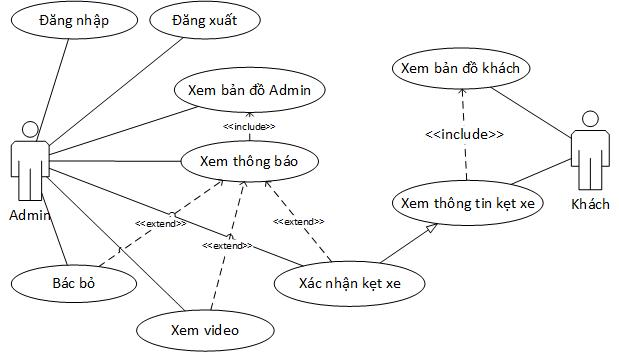
\includegraphics[scale=.75]{Graphics/usecase}
					\caption{Lược đồ Usecases}
			\end{figure}
		\end{center}

	\subsubsection{Danh sách usecases}
	
	\begin{table}[H]
		\centering
		\begin{tabularx}{\textwidth}{|c|>{\raggedright\arraybackslash}X |}
			\hline
			Tên usecase	& Mô tả\\
			\hline
			Đăng nhập&
			Quản trị viên đăng nhập bằng tài khoản có quyền admin	\\
			\hline	
			Đăng xuất	&									Đăng xuất khỏi tài khoản admin, trở lại trang chính của client\\\hline																				
			Xem bản đồ admin &										Bản đồ TPHCM biểu diễn tình hình giao thông thời gian thực, bao gồm các vị trí kẹt xe và các cảnh báo \\\hline																				
			Xem các thông báo kẹt xe&										Các cảnh báo về vị trí có khả năng sắp/đang xảy ra kẹt xe\\\hline																				
			Đồng ý thông tin kẹt xe&										Xác nhận canh báo là đúng\\\hline		
			Bác bỏ thông tin&										Bác bỏ (không xảy ra kẹt xe tại vị trí được cảnh báo)\\\hline																				
			Xem video&										Xem video được gửi về từ các camera gắn trên xe buýt\\\hline																				
			Xem bản đồ khách&										Bản đồ TPHCM biểu diễn tình hình giao thông hiện tai, bao gồm các thông báo kẹt xe\\
			\hline
			\end{tabularx}
		\caption{Danh sách các usecase}
	\end{table}
	\section{Đặc tả chi tiết các usecase}
	\subsection{Đăng nhập với tài khoản admin}
		\restylefloat{figure}
		\begin{figure}[H]
			\centering
			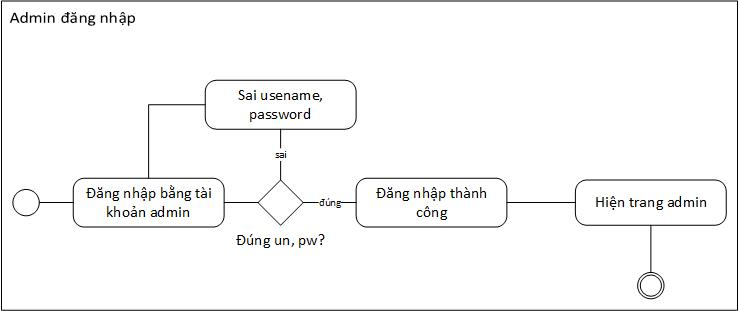
\includegraphics[scale=.75]{Graphics/activity-login}
			\caption{Activity - Đăng nhập bằng tài khoản admin}
		\end{figure}
		
	\subsection{Đăng xuất}
		\restylefloat{figure}
		\begin{figure}[H]
			\centering
			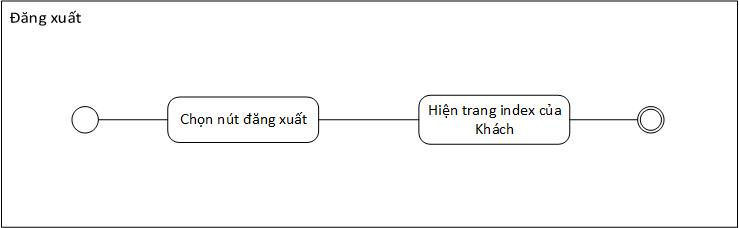
\includegraphics[scale=.75]{Graphics/activity-logout}
			\caption{Activity - Đăng xuất tài khoản admin}
		\end{figure}
				
	\subsection{Xem bản đồ admin}
		\restylefloat{figure}
		\begin{figure}[H]
			\centering
			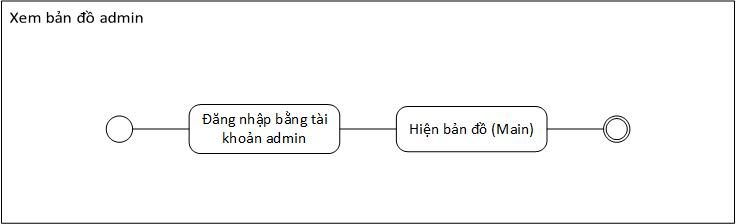
\includegraphics[scale=.75]{Graphics/activity-viewmap-admin}
			\caption{Activity - Xem bản đồ admin}
		\end{figure}
		
	\subsection{Xem các thông báo kẹt xe}
		\restylefloat{figure}
		\begin{figure}[H]
			\centering
			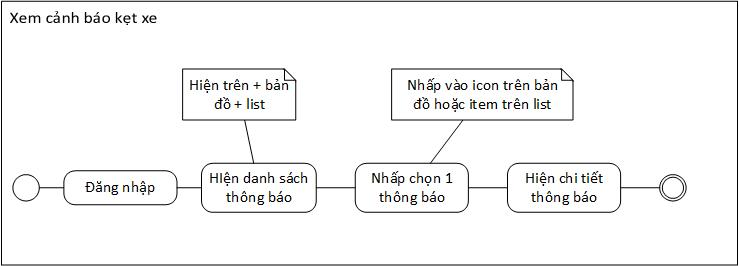
\includegraphics[scale=.75]{Graphics/activity-viewnoti}
			\caption{Activity - Xem các thông báo kẹt xe}
		\end{figure}
	
	\subsection{Đồng ý thông tin kẹt xe} 
		\restylefloat{figure}
		\begin{figure}[H]
			\centering
			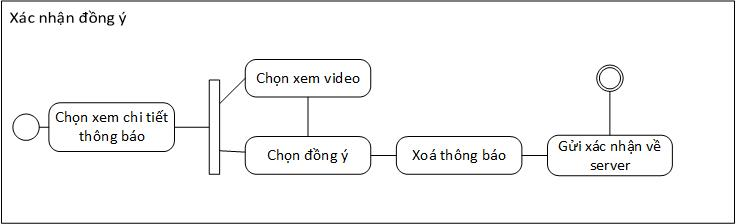
\includegraphics[scale=.75]{Graphics/activity-approve}
			\caption{Activity - Đồng ý thông tin kẹt xe}
		\end{figure}
	
	\subsection{Bác bỏ thông tin kẹt xe}
		\restylefloat{figure}
		\begin{figure}[H]
			\centering
			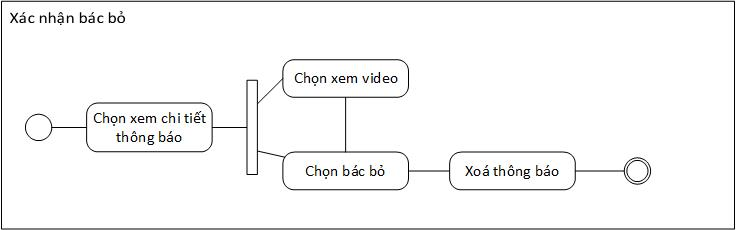
\includegraphics[scale=.75]{Graphics/activity-reject}
			\caption{Activity - Bác bỏ thông tin kẹt xe}
		\end{figure}
	
	\subsection{Xem video}
		\restylefloat{figure}
		\begin{figure}[H]
			\centering
			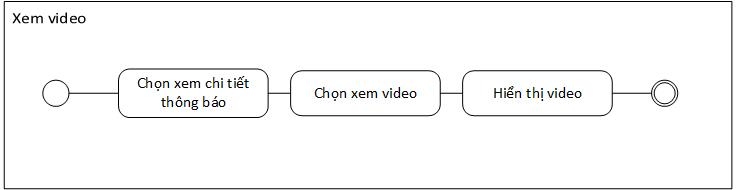
\includegraphics[scale=.75]{Graphics/activity-viewvideo}
			\caption{Activity - Xem video}
		\end{figure}
		
	
	\subsection{Xem bản đồ (khách)}
		\restylefloat{figure}
		\begin{figure}[H]
			\centering
			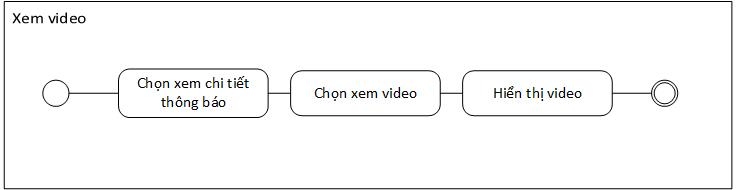
\includegraphics[scale=.75]{Graphics/activity-viewvideo}
			\caption{Activity - Xem bản đồ khách}
		\end{figure}
	
\section{Yêu cầu về giao diện người dùng}
\begin{itemize}
	\item Giao diện chính hiển thị bản đồ.
	\item Các thành phần giao diện được điều khiển bởi các trang JSP, OpenStreetMap và thư viện Leaflet, sử dụng HTML5 để hiển thị.
	\item Video và mọi nội dung khác có thể tải được trên mọi trình duyệt, đặc biệt là Internet Explorer.
	\item Sử dụng icon với nội dung cảnh báo để thể hiện thông báo về vị trí có nguy cơ kẹt xe.
	\item Sử dụng icon để thể hiện vị trí các xe buýt.
	\item Không có yêu cầu cụ thể về mỹ thuật và cách bố trí trang web.
\end{itemize}

\section{Yêu cầu về tính bảo mật}
\begin{itemize}
	\item Hệ thống được sử dụng chủ yếu bởi 2 đối tượng là khách (người dùng không đăng nhập, mọi người sử dụng internet) và người quản trị, giám sát giao thông (không phải người quản trị hệ thống). Hệ thống phải đảm bảo xác thực danh tính và quyền hạn người dùng mỗi khi họ truy cập.
	\item Một số dữ liệu của trung tâm (như các URL video) phải được che dấu đối với những người dùng không có quyền truy cập.
\end{itemize}

\section{Tài liệu hướng dẫn}
(Chưa có trong giai đoạn này.)

\section{Định hướng mở rộng}

\begin{itemize}
	\item Về tính năng:
	\subitem Tổ chức gom cụm các xe buýt xuất hiện trong một bán kính cố định hoặc tuỳ chọn (đang được cân nhắc).
	\subitem Nghiên cứu một giải thuật xác định kẹt xe có tính học thuật, dựa trên nhiều yếu tố khác ngoài vận tốc để cho ra một kết quả chính xác và có khả năng dự báo chứ không chỉ xác định. Ngoài ra, đánh giá mức độ kẹt xe.

	\item Về kỹ thuật:
	\subitem Tối ưu hỗ trợ hiển thị trên các thiết bị di động.
\end{itemize}

